\documentclass[12pt,aspectratio=169]{beamer}

\mode<presentation>
{
  \usetheme{Singapore}
  %\setbeamersize{text margin left=.6cm,text margin right=.6cm}
%  \setbeamertemplate{navigation symbols}{} % suppress nav bar
%  \setbeamercovered{transparent}
}
\usefonttheme{professionalfonts}
\usepackage{graphicx}
\usepackage{tikz}
\usepackage{amsmath}
\usepackage{mathpazo}
\usepackage[scaled]{helvet}
\usepackage{xcolor,colortbl}
\usepackage{siunitx}

\sisetup{number-math-rm=\mathnormal}

\title{Class 11: Gauss's Law and Other Wonderful Topics}
\subtitle{AP Physics}
\author[TML]{Dr.\ Timothy Leung}
\institute{Olympiads School}
\date{February 2018}

\newcommand{\pic}[2]{\includegraphics[width=#1\textwidth]{#2}}
\newcommand{\mb}[1]{\mathbf{#1}}
\newcommand{\eq}[2]{\vspace{#1}{\Large\begin{displaymath}#2\end{displaymath}}}


\begin{document}

\begin{frame}
  \maketitle
\end{frame}


\section[Intro]{Introduction}

\begin{frame}
  \frametitle{Files for You to Download}
  Download from the school website:
  \begin{enumerate}
  \item\texttt{11-Gauss.pdf}---This presentation. If you want to print
    on paper, I recommend printing 4 pages per side.
  \item\texttt{11-Homework.pdf}---Homework assignment for this class.
  \end{enumerate}

  \vspace{.2in}
  Please download/print the PDF file before each class. There is no point
  copying notes that are already printed out for you. Instead, take notes on
  things I say that aren't necessarily on the slides.
\end{frame}



\section{Charge Distributions}

\begin{frame}
  \frametitle{Electric Field from Charge Distributions}

  From last class (and Physics 12), we know that the electric field from a
  point charge $q$ is given by:

  \eq{-.2in}{\mb{E}=\frac{kq}{r^2}\hat{\mb{r}}}
  
  where $\hat{\mb{r}}$ is the outward radial direction from the charge. The
  total field at a point $P$ from a distribution of charge is found by
  integrating through the entire volume of the charge:

  \eq{-.2in}{\boxed{\mb{E}=\int_V\frac{kdq}{r^2}\hat{\mb{r}}}}
\end{frame}


%\begin{frame}
%  \frametitle{Electric Field Along Bisector of a Finite Line Charge}
%  \begin{columns}
%    \column{.3\textwidth}
%    \pic{1}{thinrod.jpg}
%    \column{.7\textwidth}
%    \begin{itemize}
%    \item A thin rod with length $\ell$, and charge distribution $\lambda$
%    \item The parallel component $dE_x$ does not contribute, but
%      perpendicular component $dE_y$ does:
%
%      \eq{-.2in}{
%        dE_y=\frac{k dq}{r^2}\cos\theta
%        =\frac{k\lambda dx}{r^2}\cos\theta
%      }
%    \item We integrate through the 
%    \end{itemize}
%  \end{columns}
%\end{frame}
%
%
%\begin{frame}
%  \frametitle{Infinite Line Charge}
%  
%\end{frame}


\begin{frame}
  \frametitle{Electric Field Along Axis of a Ring Charge}
  You're Given The One Ring To Rule Them All\ldots what is its electric
  field at point $P$ along its axis?

  \begin{center}
    \pic{.65}{physicsbook_emism_graphik_35.png}
  \end{center}
\end{frame}


\begin{frame}
  \frametitle{Electric Field Along Axis of a Ring Charge}
  \begin{columns}
    \column{.3\textwidth}
    \pic{1.25}{Fig25.jpg}
%    \eq{.05in}{r^2=x^2+a^2}
    \column{.7\textwidth}
    \begin{itemize}
    \item We can separate the electric field $d\mb{E}$ from charge $dq$ into
      axial ($dE_x$) and radial ($dE_\perp$) components
    \item From symmetry, $dE_\perp$ doesn't do contribute to anything; but
      $dE_x$ is pretty easy to find:

    \end{itemize}
  \end{columns}
  \eq{.05in}{
    dE_x =\frac{kdq}{r^2}\cos\theta=\frac{kdq}{r^2}\frac{x}{r}
    =\frac{kxdq}{(x^2+a^2)^{3/2}}
  }      
  Integrating this over all charges $dq$, we have:
  
  \eq{-.2in}{
    E_x =\frac{kx}{(x^2+a^2)^{3/2}}\int dq=\boxed{\frac{kQx}{(x^2+a^2)^{3/2}}}
  }
\end{frame}




\begin{frame}
  \frametitle{Electric Field Along Axis of a Uniformly Charged Disk}
  Let's extend what we know to a disk of radius $R$ and charge density $\sigma$
  \begin{columns}
    \column{.3\textwidth}
    \pic{1.2}{serway.png}
    \column{.67\textwidth}
    \begin{itemize}
    \item We start with the solution from the ring problem, and replace $Q$
      with $dq=2\pi\sigma a da$:

      \eq{-.2in}{
        dE_x =\frac{2\pi kx\sigma ada}{(x^2+a^2)^{3/2}}
      }
    \item Integrating over the entire disk:

      \eq{-.3in}{
        E_x =\pi kx\sigma\int\frac{2ada}{(x^2+a^2)^{3/2}}
      }

      \vspace{-.15in}This is not an easy integral!
    \end{itemize}
  \end{columns}
\end{frame}



\begin{frame}
  \frametitle{Eclectic Field Along Axis of a Uniformly Charged Disk}
  \begin{columns}
    \column{.3\textwidth}
    \pic{1.2}{serway.png}
    \column{.67\textwidth}
    \begin{itemize}
    \item Luckily for us, the integral is in the form of $\int u^ndu$, with
      $u=x^2+a^2$ and $n=\frac{-3}{2}$.
    \item You can find the integral in any math textbook:

      \eq{-.3in}{
        \boxed{E_x =2\pi k\sigma\left(1-\frac{x}{\sqrt{x^2+R^2}}\right)}
      }
      \end{itemize}
  \end{columns}
\end{frame}

\section{Gauss's Law}

\begin{frame}
  \frametitle{Flux}

  \textbf{Flux} is an important concept in many disciplines in physics. The
  flux of a vector quantity $\mb{X}$ is the amount of that quantity flowing
  through a surface. In integral form:

  \eq{-.2in}{\Phi=\int\mb{X}\cdot d\mb{A}}

  The direction of the infinitesimal area $d\mb{A}$ is \textbf{outward normal}
  to the surface.

  \begin{center}
    \pic{.3}{eflux.png}
  \end{center}
\end{frame}

\begin{frame}
  \frametitle{Flux}
  \vspace{.2in}$\Phi$ can be something very physical, like water, or bananas, or
  something abstract, like electric field (which is what we are interested
  in). We can compute a flux as long as there is a vector field i.e.\
  $\mb{X}=\mb{X}(x,y,z)$.
  In the case of \textbf{electric flux}, the quantity $\mb{X}$ is just the
  electric field, i.e.:
    
  \eq{-.2in}{\Phi_\mathrm{electric}=\int\mb{E}\cdot d\mb{A}}
  
  \begin{center}
    \pic{.3}{eflux.png}
  \end{center}
\end{frame}

\begin{frame}
  \frametitle{Electric Flux and Gauss's Law}
    \textbf{Gauss's law} tells us that if we have a closed surface (think of
    the surface of a balloon), the total electric flux is very well defined:

    \eq{-.2in}{\boxed{
        \Phi_\mathrm{total}
        =\oint\mb{E}\cdot d\mb{A}
        =\frac{Q_\mathrm{encl}}{\epsilon_0}
    }}
    
    \vspace{-.1in}where $Q_\mathrm{encl}$ is the charge enclosed by the surface,
    and $\epsilon_0=\SI{8.85e-12}{C^2/N.m^2}$ is the permittivity of free space.
    That closed surface is called a \textbf{Gaussian surface}.
\end{frame}


\begin{frame}
  \frametitle{Electric Field from a Positive Point Charge}
  
  \begin{columns}
    \column{.25\textwidth}
    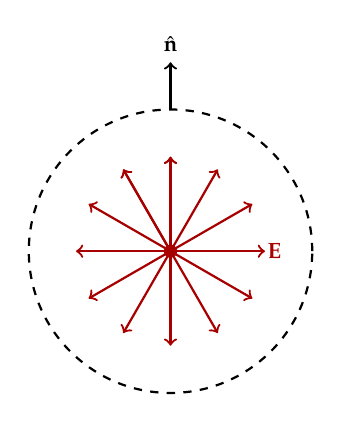
\begin{tikzpicture}[scale=1.2]
      \fill[red!65!black](0,0) circle(0.07);
      \draw[dashed,thick](0,0) circle(1.5);
      \foreach \x in {0,...,13}{
        \draw[red!65!black,thick,rotate=30*\x,->](0,0)--(0,1);
      }
      \draw[thick,->](0,1.5)--(0,2)
      node[pos=1,above]{\footnotesize$\hat{\mb{n}}$};
      \node[red!65!black] at (1.1,0) (E) {\footnotesize$\mb{E}$};
    \end{tikzpicture}
    \column{.75\textwidth}
    By symmetry, electric field lines are radially outward from the charge, so
    the integral reduces to:

    \eq{-.2in}{\Phi=\oint\mb{E}\cdot d\mb{A}=EA=\frac{q}{\epsilon_0}}

    And since area of the sphere is just $A=4\pi r^2$, we recover Coulomb's law:

    \eq{-.3in}{ E=\frac{1}{4\pi\epsilon_0}\frac{q}{r^2}=\frac{kq}{r^2}}
    
    In fact, it was through studying point charges that Gauss's law was
    discovered, so it should not be a surprise that they agree.
  \end{columns}
\end{frame}


\begin{frame}
  \frametitle{In Your Homework This Week}
  In the homework questions this week, you will be asked to find the
  electric field strength inside and outside of a few common configurations:
  \begin{itemize}
  \item Inside \& outside of a spherical shell of charge
  \item Inside \& outside of a uniformly charged solid sphere
  \item Near an infinite line charge
  \item Inside \& outside an infinitely long solid cylinder of charge
  \item Inside \& outside a cylindrical shell of charge
  \end{itemize}
\end{frame}


\begin{frame}
  \frametitle{Electric Field Near an Infinite Plane of Charge}
  \begin{columns}
    \column{.25\textwidth}
    \pic{1.3}{elec_gauss_figure9.jpg}
    \column{.75\textwidth}
    \begin{itemize}
    \item Charge density (charge per unit area) $\sigma$
    \item By symmetry, $\mb{E}$ must be perpendicular to the plane
    \item Our Gaussian surface is a cylinder shown in the left with an area
      $A$; the height of the cylinder is unimportant
    \item We can see that nothing ``flows out'' of the side of the cylinder,
      only at the ends.
    \item The total flux is $\Phi=E(2A)$
    \item The enclosed charge is $Q_\mathrm{encl}=\sigma A$.
    \end{itemize}
  \end{columns}
%  \vspace{.5in}{\tiny Diagram from Paul A.\ Tipler,
%    \emph{Physics for Scientists and Engineers, Volume 2}, Third Edition, Worth
%    Publisher, New York, 1991.}
\end{frame}


\begin{frame}
  \frametitle{Electric Field Near an Infinite Plane of Charge}
  \begin{columns}
    \column{.25\textwidth}
    \pic{1.3}{elec_gauss_figure9.jpg}
    \column{.75\textwidth}
    Gauss's law simplifies to:
    
    \eq{-.35in}{
      \oint\mb{E}\cdot d\mb{A}=\frac{Q_\mathrm{encl}}{\epsilon_0}
      \;\;\rightarrow\;\;
      E(2A)=\frac{\sigma A}{\epsilon_0}
    }

    Solving for $E$, we get:

    \eq{-.3in}{\boxed{E=\frac{\sigma}{2\epsilon_0}}}
    \begin{itemize}
    \item $E$ is a constant
    \item Independent of distance from the plane
    \item Both sides of the plane are the same
    \end{itemize}
  \end{columns}
\end{frame}



\begin{frame}
  \frametitle{Electric Field Between Parallel Charged Plates}
  Remember being told that the electric field between two charged plates
  is constant?

  \begin{itemize}
  \item Two plates, each producing an electric field pointing in the same
    direction
  \item The total electric field is twice the value that we found on the last
    slide

    \eq{-.1in}{\boxed{E=\frac{\sigma}{\epsilon_0}}}

    which is what we already know!
  \end{itemize}
\end{frame}




\section{Capacitors}


\begin{frame}
  \frametitle{Capacitors}
  \textbf{Capacitors} stores energy in a circuit. The
  simplest form of a capacitor is a set of closely spaced parallel plates:

  \begin{center}
    \pic{.5}{cap19.png}%{pplate.jpg}
  \end{center}
  
  When the plates are connected to a battery, the battery transfer charges to
  the plates until the potential difference (voltage) $V$ equals the battery
  terminals. At that time, the plates has charge $+Q$ on one side, and $-Q$ on
  the other.
%  \vspace{.5in}{\tiny Diagram from Paul A.\ Tipler,
%    \emph{Physics for Scientists and Engineers, Volume 2}, Third Edition, Worth
%    Publisher, New York, 1991.}
\end{frame}

\begin{frame}
  \frametitle{Parallel Capacitors}
  Since we know what $E=\sigma/\epsilon_0$ between the plates, and the
  relationship $E=V/d$, we can relate $V$ to the amount of charge $Q$ stored
  between the plates:

  \eq{-.2in}{ V=Ed=\frac{\sigma}{\epsilon_0}d=\frac{Qd}{\epsilon_0A}}

  The ratio between charge $Q$ and voltage $V$ is defined as the
  \textbf{capacitance} $C$:

  \eq{-.2in}{
    \boxed{C=\frac{Q}{V}}
    \quad\quad
    \text{\normalsize for parallel plates:}
    \;\;
    C=\frac{\epsilon_0A}{d}
    \;\;\text{\normalsize (constant!)}
  }
\end{frame}


\begin{frame}
  \frametitle{Capacitors}

  Capacitance $C$ is defined as the ratio between charge $Q$ and potential
  difference (voltage) $V$:
  
  \eq{-.05in}{
    \boxed{C=\frac{Q}{V}}
  }
  
  \begin{center}
    \begin{tabular}{l|c|l}
      \rowcolor{pink}
      \textbf{Quantity} & \textbf{Symbol} & \textbf{SI Unit} \\ \hline
      Capacitance   & $C$   & \si{\farad} (farads)\\
      Charge        & $Q$   & \si{\coulomb} (coulombs)\\
      Voltage across the plates & $V$ & \si{\volt} (volts)
    \end{tabular}
  \end{center}

\end{frame}

\begin{frame}
  \frametitle{Real Capacitors}
  \begin{columns}
    \column{.25\textwidth}
    \pic{1.2}{Figure_20_05_05a.jpg}
    \column{.75\textwidth}
    \begin{itemize}
    \item Parallel-plate capacitors are very common in electric circuits,
      but a vacuum between the plates is not very effective
    \item Instead, a \textbf{dielectric} (nonconducting) material is inserted
      between the plates
    \item When the plates are charged, the electric field of the plates
      polarizes the dielectric.
    \item The dielectric now produces an electric field that opposes the field
      from the plates, therefore reduces the effective voltage, and increasing
      the capacitance
    \end{itemize}
  \end{columns}
\end{frame}


\begin{frame}
  \frametitle{Dielectric Constant}
  \begin{columns}
    \column{.65\textwidth}
    If electric field without dielectric is $E_0$, then $E$ in the
    dielectric is reduced by $\kappa$, the \textbf{dielectric constant}:

    \eq{-.25in}{\boxed{E=\frac{E_0}{\kappa}}}

    \vspace{-.1in}The capacitance in a dielectric is now amplified:

    \eq{-.25in}{\boxed{C=\kappa C_0}}

    \vspace{-.15in}We can also view the dielectric as something that
    increases the effective permittivity:

    \eq{-.3in}{\boxed{\epsilon=\kappa\epsilon_0}}

    \column{.35\textwidth}
    \begin{tabular}{l|l}
      \rowcolor{pink}
      \textbf{Material} & $\kappa$ \\ \hline
      Air         & \num{1.00059} \\
      Bakelite    & \num{4.9} \\
      Pyrex glass & \num{5.6} \\
      Neoprene    & \num{6.9} \\
      Plexiglas  & \num{3.4} \\
      Polystyrene & \num{2.55} \\
      Water (\SI{20}{\celsius}) & \num{80} 
    \end{tabular}
    \end{columns}
\end{frame}


\begin{frame}
  \frametitle{Storage of Electrical Energy}
  \begin{center}
    \pic{.45}{slide14.jpg}
  \end{center}

  \begin{itemize}
  \item When charging up a capacitor, imagine positive charges moving from the
    negatively charged plate to the positively charged plate
  \item Initially neither plates are charged, so moving the first charge takes
    very little work; as the electric field builds, more and more work needs
    to be done
  \end{itemize}
\end{frame}

\begin{frame}
  \frametitle{Storage of Electrical Energy}

  Starting from the beginning, if we move an infinitesimally charge $dq$
  across the plate, the infinitesimal work done $dU$ is related to the
  capacitance:

  \eq{-.22in}{dU=Vdq=\frac{q}{C}dq}

  \vspace{-.1in}To fully charge the plates, the total work $U$ is the integral:

  \eq{-.2in}{U=\int dU=\int_0^Q\frac{q}{C}dq=\frac{1}{2}\frac{Q^2}{C}}

  There are different ways to express $U$ using definition of capacitance:

  \eq{-.2in}{\boxed{U=\frac{1}{2}\frac{Q^2}{C}=\frac{1}{2}QV=\frac{1}{2}CV^2}}
\end{frame}
\end{document}
